\chapter{Overview and Evaluation of the Exergame}\label{chapter:finaldesign}
The overall exergame development was user centred. Based on the feedback gathered from the prototype game review, discussions with experts, and literature review, new movements have been introduced and modifications have been made to the existing design in order to make the exergame engaging, enjoyable, and more intuitive to use and interact with for the future users. This section outlines the design and development of the final version of the Immotion exergame for warm up routine guidance and motivation.
\section{A Modular Design Approach}
In order to make the exergame easily adjustable and compliant with the user requirements, in our exergame design and development we followed a modular design approach. That is, each movement (exercise) that was required from the user has been encapsulated in one distinct game segment. To put it differently, the whole game system was subdivided into smaller parts that could be independently created and then used accordingly. That way, by combining multiple segments randomly, we were able to generate a unique game map each time the user played the exergame. The end result of this approach was that our game is not constrained by one global map, but a dynamic one created on each game run. Moreover, having segments as the basic game blocks allowed us to easily add new segments that could make the game richer and the set of required movements bigger. Also, this way we could easily update or discard segments and movements users disliked or were difficult to perform. We believe this is a major feature that made our exergame scalable and extensible for future user requirements and preferences. 
\section{Discussions With Fitness Experts}
During the development of our exergame, fitness and exercise experts were consulted in order to design game segments that would require movements often performed before physical activity and be effortlessly executed by the users without prior exercise knowledge. \\Based on the comments received by the experts, we modified existing segments so the movements that are required to be executed are more intuitive for the user and do not require further explanation. The modular design approach allowed us to easily add segments that required movements suggested by the experts at the spot and modify existing ones. Suggestions and additional features recommended by experts were taken into account while designing all the game segments used in the final version of the exergame.  Figure \ref{fig:expDesign} captures one of our discussion with the fitness expert.\\  
 \begin{figure}[h]
    \centering
    \includegraphics[width=\textwidth]{expertsDesign}
    \caption{Exergame related design discussion with the fitness expert.}
    \label{fig:expDesign}
\end{figure}\\
In the next sections we describe and present the redesigned exergame, the new segments introduced, as well as the movements that were required to be performed within them.\pagebreak
\section{Coins Overview}
For the final version of the exergame, we extended the set of coins the player can collect during the gameplay. Compared to the previous exergame version presented in Figure \ref{fig:points}, three new types of coins were made available to the players. Figure \ref{fig:new_coins} summarizes the available coin types.  
\begin{figure}[h]
    \centering
    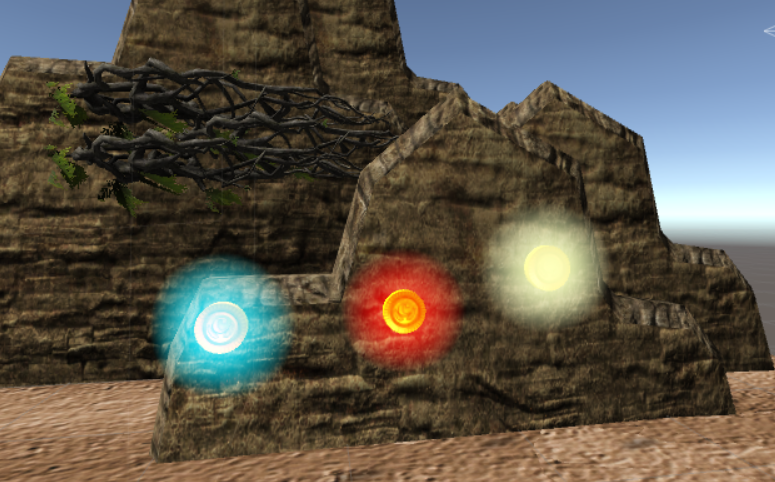
\includegraphics[width=\textwidth]{new_coins}
    \caption{Coin types available in the exergame.}
    \label{fig:start}
\end{figure}\\
Each coin type presented in Figure \ref{fig:new_coins}  was worth different amount of points. How much point each coin was worth is as follows:
\begin{itemize}
\item Yellow coin - 1 point.
\item Red coin - 3 points.
\item Blue coin - 5 points.
\end{itemize}
We positioned the coins in the segments in a way the player could chose between two options. First one was to collect less points without any possibility to hit an obstacle, The second was to collect more points, but the chance to hit an obstacle and lose points, was much higher. This way we hoped to provide players the \textit{autonomy} over their own actions and decisions as much as possible. This can, as per \acrshort{sdt}, impact ones intrinsic motivation. 
\section{Home Window Overview}
When the user starts the exergame, the \textit{Home screen} that is depicted in Figure \ref{fig:start} is showed. Apart from starting the game, other options are available for the user as well:
\begin{itemize}
\item Start
\item Help
\item Volume
\item High Score
\item Quit
\end{itemize}
\begin{figure}[h]
    \centering
    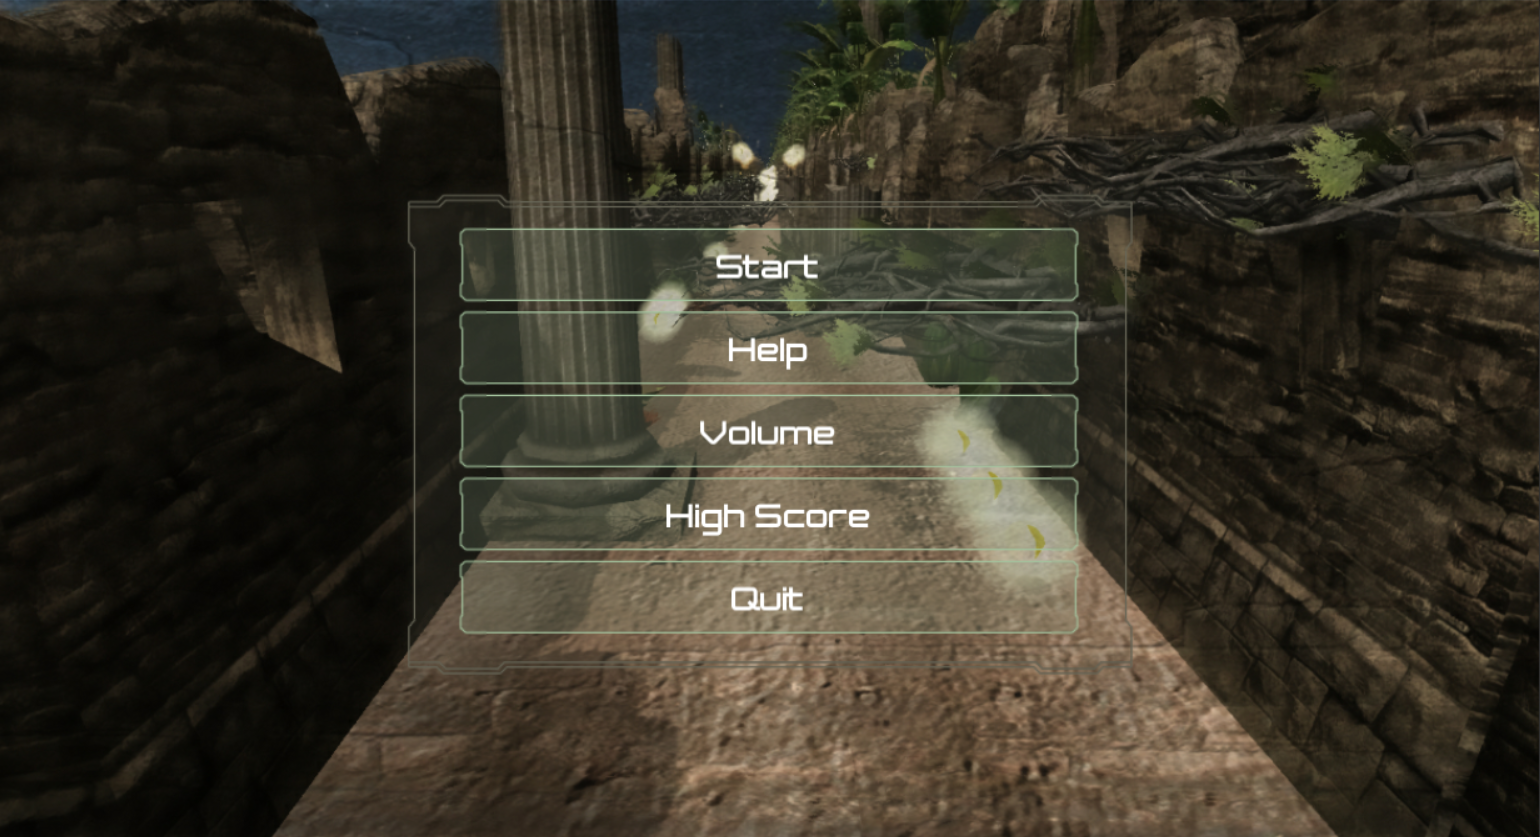
\includegraphics[width=\textwidth]{Start}
    \caption{Home screen.}
    \label{fig:start}
\end{figure}
Each of the above presented options opens a new window and provides the user with certain functions. Next, the above listed options will be further detailed.\pagebreak
\paragraph{Start Menu}
By selecting the \textit{Start} button in the Home screen, the user is presented with a new screen as showed in Figure \ref{fig:userinfo}. In this step, the user needs to input a username that will be used throughout the gameplay. The username does not have to be unique. In case it already exists, at the end of the game, all the scores achieved in previous game runs with the same username will be presented in descending order by game scores as showed in Figure \ref{fig:individualScore}. By selecting the Start button the exergame begins. By selecting the \textit{Back} button, the user is directed back to the Home screen.\\
\begin{figure}[h]
    \centering
    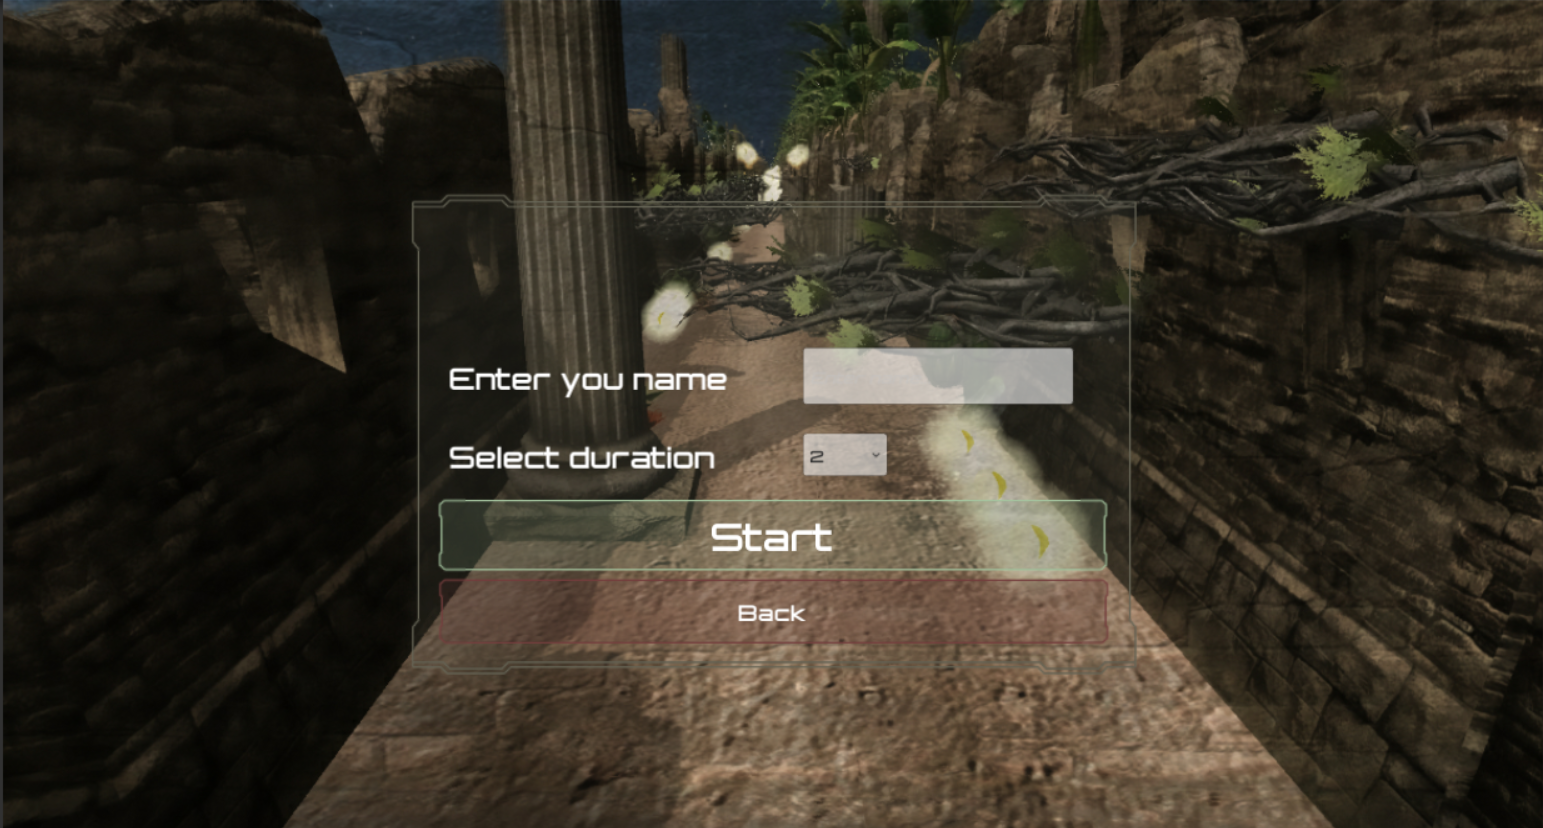
\includegraphics[width=\textwidth]{EnterName}
    \caption{Userrname Input menu.}
    \label{fig:userinfo}
\end{figure}
\paragraph{Help Menu}
The Help menu, as presented in Figure \ref{fig:help} lets the user know how to interact with the game, change the speed of the game, and start or stop the game. It also contains contact information for error reporting and user feedback. The Back button allows the user to go back to the Home screen.
\begin{figure}[h]
    \centering
    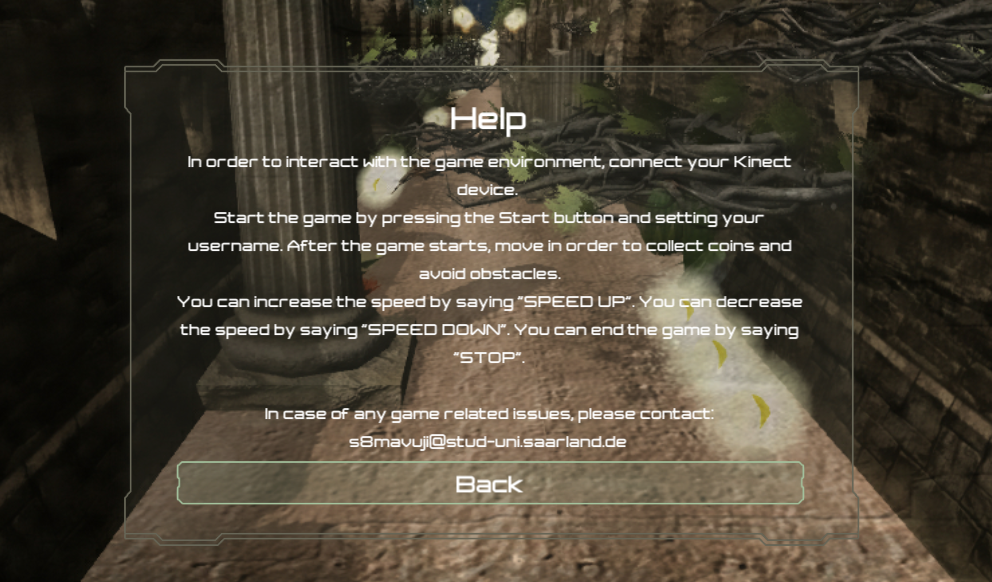
\includegraphics[width=\textwidth]{Help}
    \caption{Help menu.}
    \label{fig:help}
\end{figure}
\paragraph{Volume Menu}
The volume menu showed in Figure \ref{fig:volume}, gives users the possibility to modify the volume of the exergame's background music and sound effects (coins and obstacle collision sounds).\\
\begin{figure}[h]
    \centering
    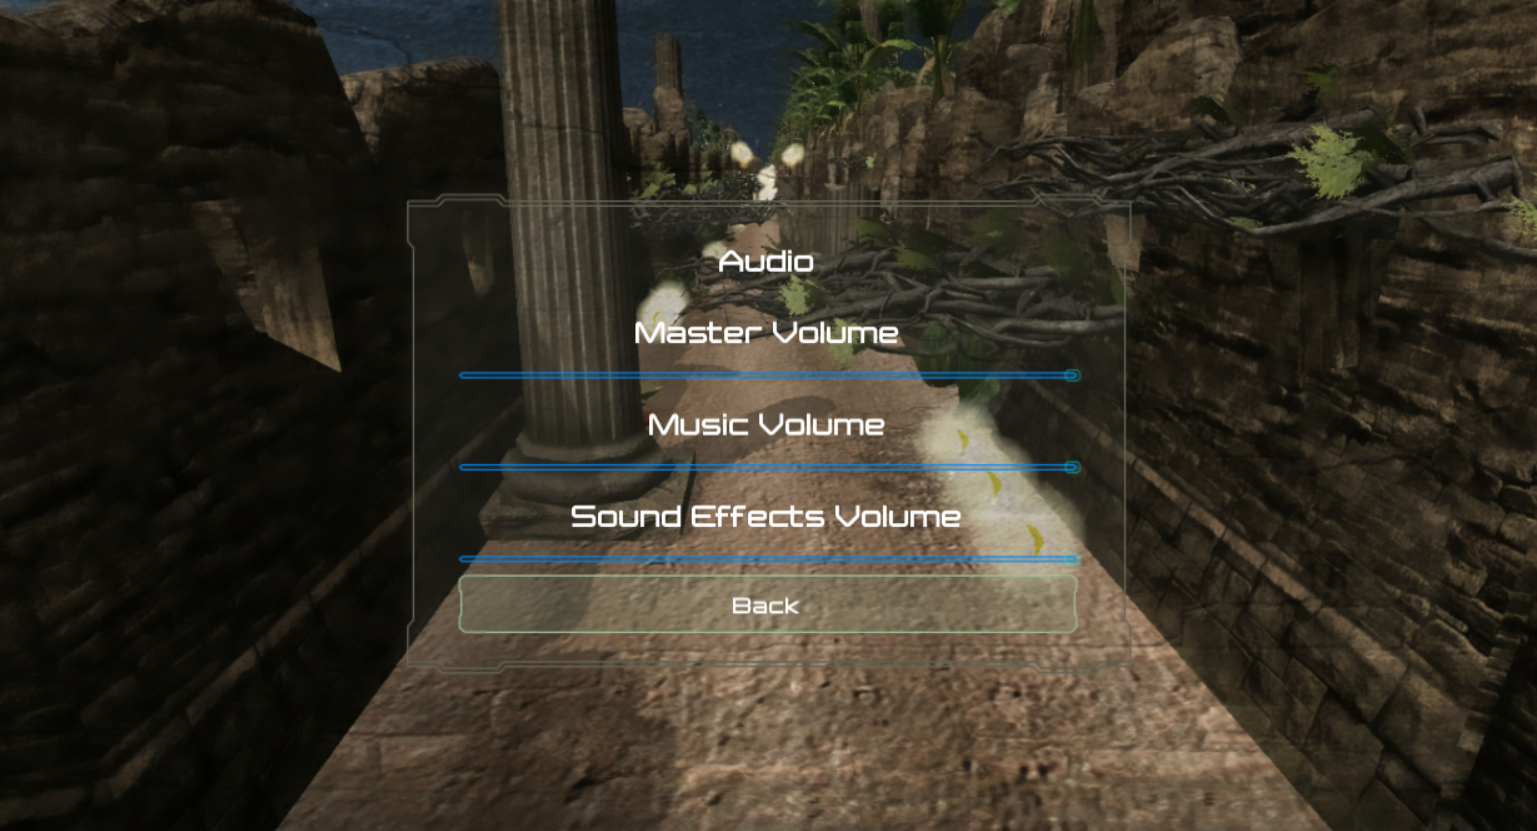
\includegraphics[width=\textwidth]{Volume}
    \caption{Adjust volume menu.}
    \label{fig:volume}
\end{figure}
\paragraph{High Score Menu}
The high score menu depicted in Figure \ref{fig:highscore} ranks the users who played the exergame based on the points collected during one gameplay. The leaderboard displays the user's rank, name, score, and duration. This is a global leaderboard and it is different than the one presented in Figure \ref{fig:individualScore} since it includes all the users previously interacted with the game, their scores, and duration they played the game. Contrarily, the individual score board, displayed only at the end of each gameplay, shows the score and game duration of the user who currently interacted with the exergame. The Back button allows the user to go back to the Home screen.TODO!
\begin{figure}[h]
    \centering
    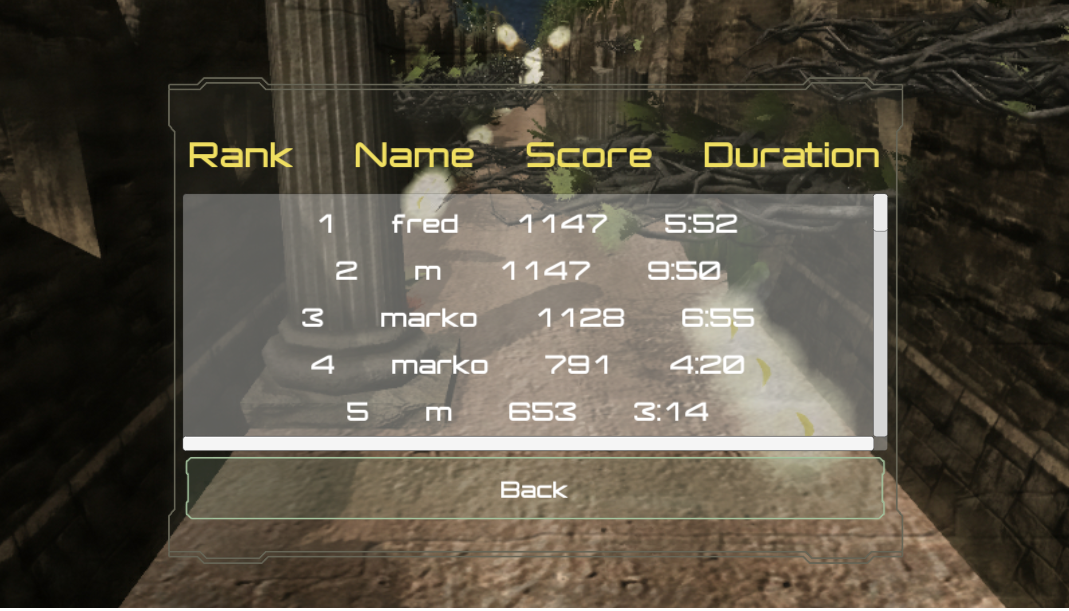
\includegraphics[width=\textwidth]{HighScore}
    \caption{High score menu.}
    \label{fig:highscore}
\end{figure}
\paragraph{Quit Menu}
The quit menu button was used for ending (closing) the game. 
\section{Game Start Overview}
For the purpose of tracking progress and achievements over time, users were required to input a name or username they would like to use during the gameplay. Based on the username, we displayed the user's current score and position on the leaderboard during the gameplay, and the highest scores at the end of the gameplay. \\The live score board and the leaderboard are presented in Figure \ref{fig:livescore} and Figure \ref{fig:highscore}. After the user set the username and pressed the Start button, a \textit{Countdown window} as showed in Figure \ref{fig:counter} is first displayed. The duration of the countdown is set to 5 seconds. We opted for this duration because it showed as the most optimal in our pilot study previously conducted with the university personal and the fitness expert. This amount of time was sufficient for the users to prepare for the upcoming exercise by moving to the correct position. In case the user was not in the Kinect sensor range at the beginning of the game, a popup information window was displayed as showed in Figure  \ref{fig:waiting}. This information window was also displayed in case the connection to the Kinect sensor failed during the gameplay. \\
\begin{figure}[h]
    \centering
    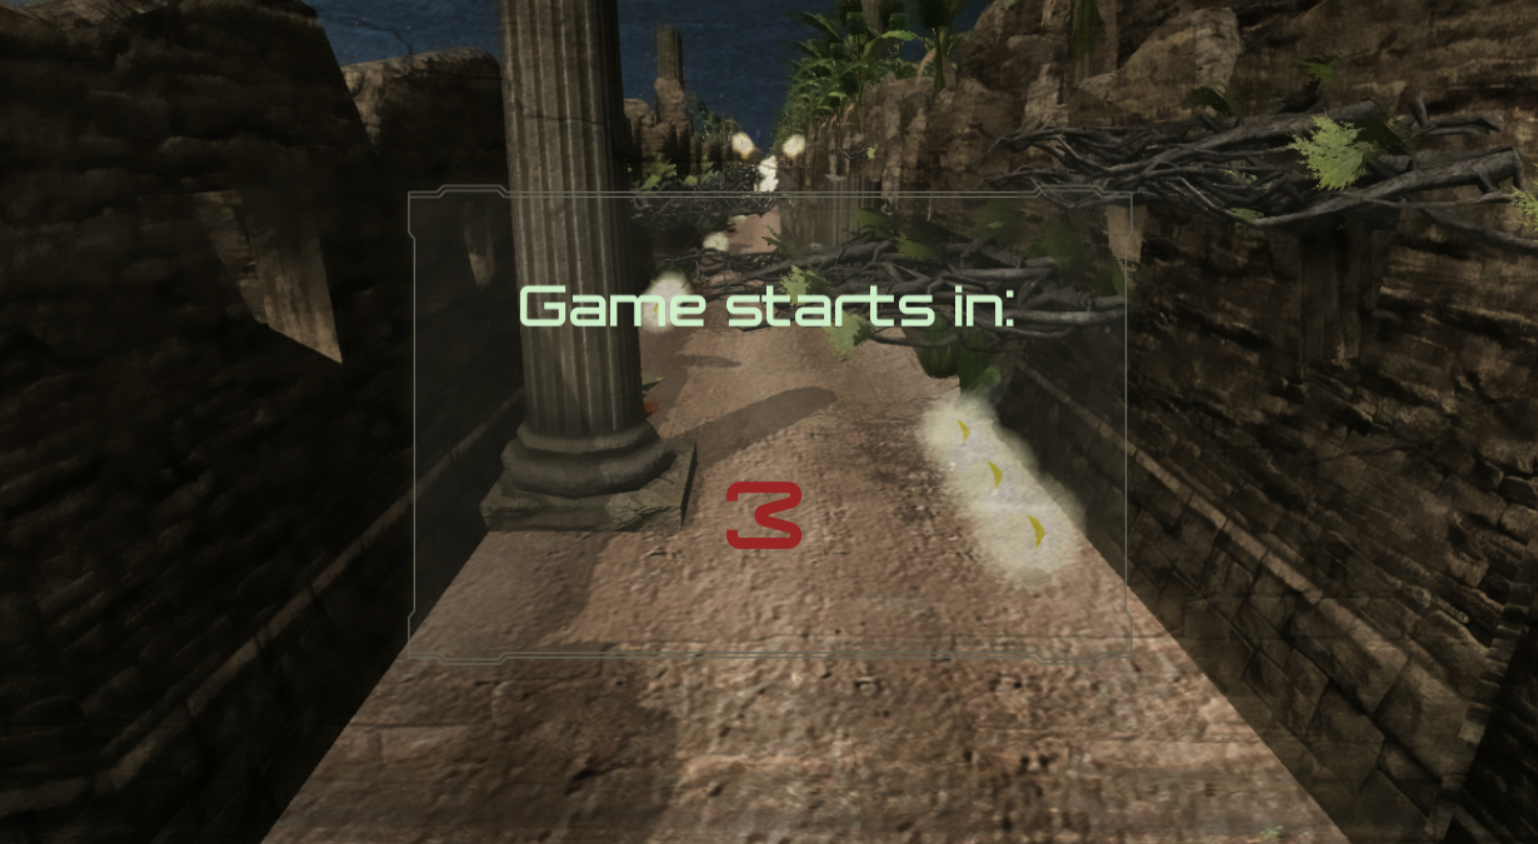
\includegraphics[width=\textwidth]{Counter}
    \caption{Countdown window.}
    \label{fig:counter}
\end{figure}\\
\begin{figure}[h]
    \centering
    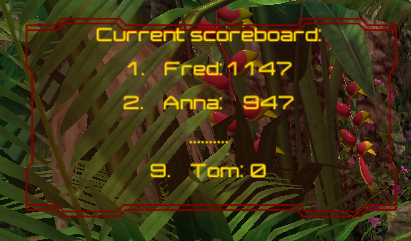
\includegraphics[width=0.6\textwidth]{LiveScore}
    \caption{``Live score'' during gameplay displayed in the left corner.}
    \label{fig:livescore}
\end{figure}\\
\begin{figure}[h]
    \centering
    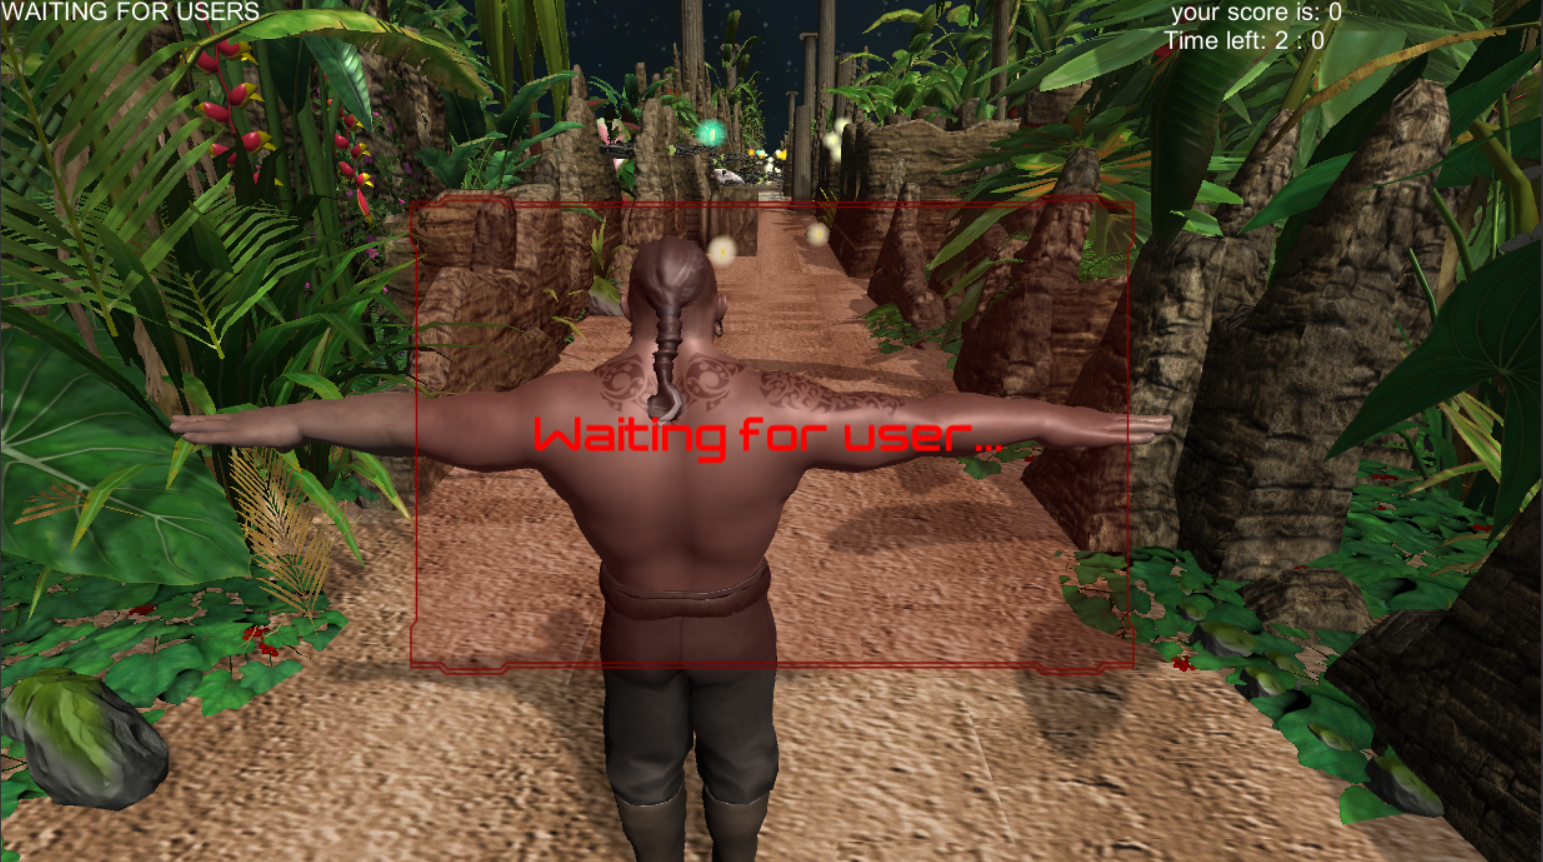
\includegraphics[width=\textwidth]{WaitingForUser}
    \caption{``Waiting for the user'' popup window.}
    \label{fig:waiting}
\end{figure}\\
Next, an overview of the game segments and corresponding movements required to perform in each of them will be presented.
\section{Game Segments Overview}
As already pointed out, each warm up movement the user was required to perform has been represented by a game segment. Following recommendations from experts, available literature, and the previously conducted online study, the list of warm up movements the users were required to perform during the game was updated. Additionally, we introduced so called \textit{filler} or \textit{empty} segments. In these segments no movements were required to be performed. They were placed between regular segments where movements needed to be performed. Their only purpose was to give users a short amount of time to prepare for the subsequent game segment. By generating all the segments randomly during gameplay, each resulting game map and warm up session induced by the map were unique. Moreover, our intention was to make the exergame intuitive to use. That is, the movements should come naturally to the users and should not require additional explanation. This was the result of our iterative and user centered design approach. We designed the segments based on the movements that can help users to warm up, and not contrarily. That way, every movement induced by obstacles and coins was executed correctly and came naturally to the player without additional explanation. Figure \ref{fig:topview} gives an overview of all the segments used in the exergame.\pagebreak
\begin{figure}[h]
    \centering
    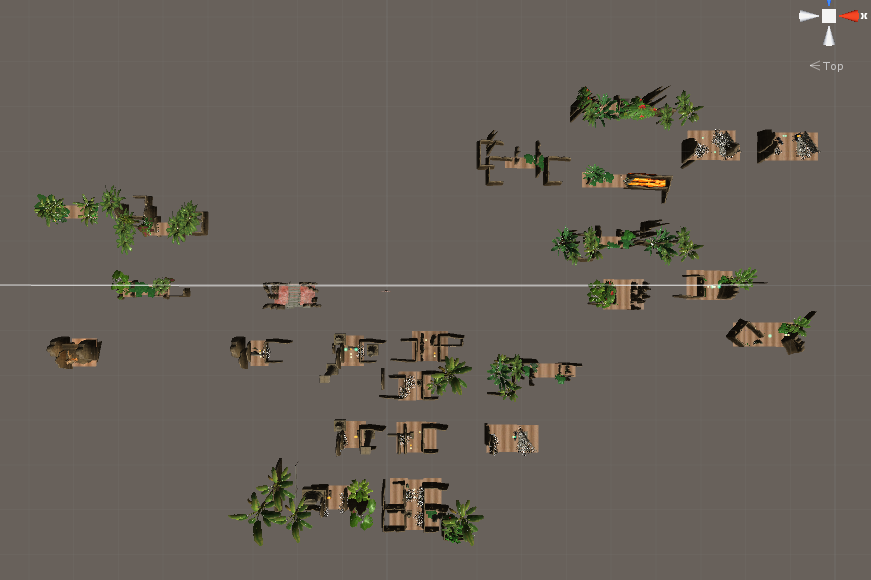
\includegraphics[width=\textwidth]{SegmentsTopView}
    \caption{Overview of game segments - top view.}
    \label{fig:topview}
\end{figure}\\
In most of the segments depicted in Figure \ref{fig:topview}, one specific movement was required to be performed. Some segments were without obstacles and were present in order for the users to prepare for the next segment (and movements). Also, segments without any obstacles were used at the beginning of the exergame. During the experiments, ten filler segments were generated at the beginning of every game run. However, this number has been made adjustable. The empty segments were placed at the beginning in order to avoid any sudden movements by the player risking injuries. Moreover, not having to perform any movements gave the player time to adjust to the gameplay and prepare for the movements. All the segments were designed to induce one of the following movement:
\begin{itemize}
\item Left hand up
\item Right hand up
\item Squat (short and long)
\item Jump
\item Star jump
\item Left hand down to the floor
\item Right hand down to the floor
\end{itemize}
Figure \ref{fig:rightup} shows the segment in which the user was required to move the right hand in the upper position and, in the same time, avoid the obstacle. In case the user came in contact with the obstacle, one point was substracted from the overall user's score.\\
\begin{figure}[h]
    \centering
    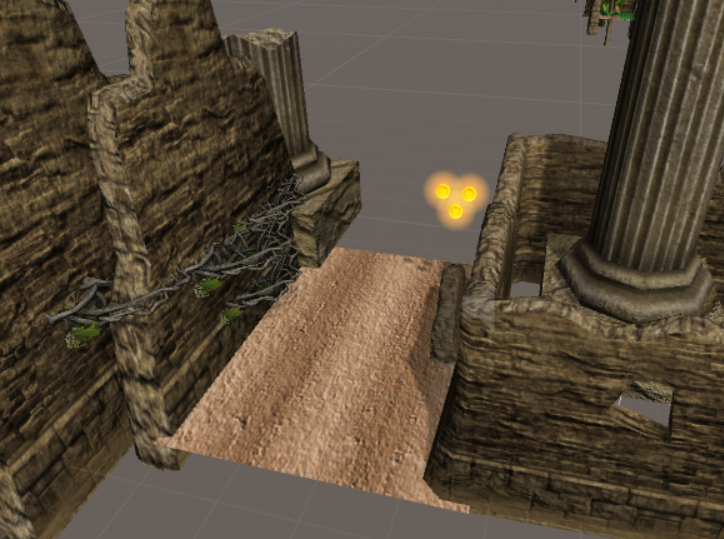
\includegraphics[width=0.85\textwidth]{RightHandUp}
    \caption{Right hand up segment.}
    \label{fig:rightup}
\end{figure}
\begin{figure}[h]
    \centering
    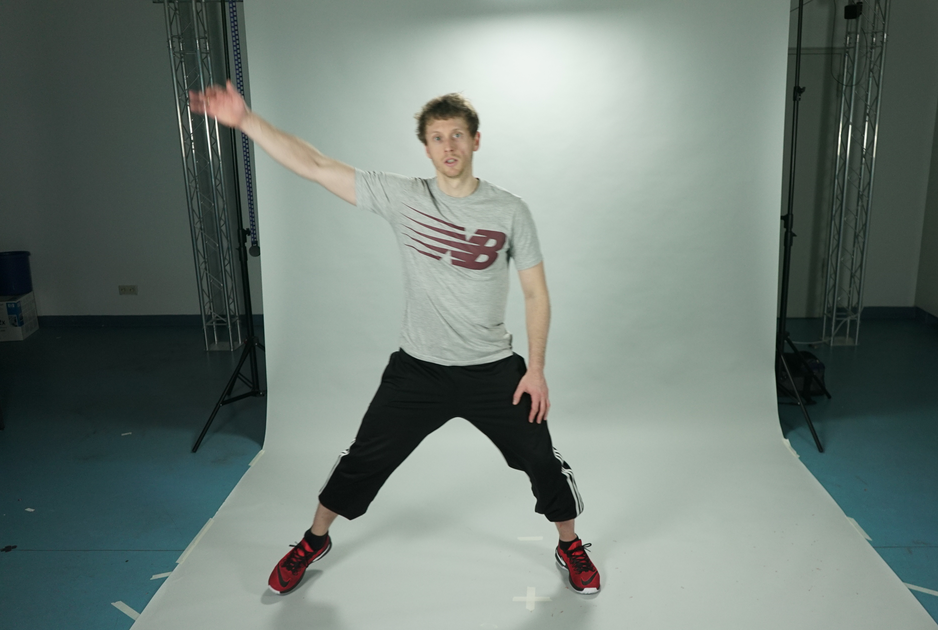
\includegraphics[width=0.85\textwidth]{ExpertRightHandUp}
    \caption{Expert right hand up movement.}
    \label{fig:expertRightHandUp}
\end{figure}\\\\
Figure \ref{fig:leftup} depicts the segment in which the user is required to move the left hand in the upper position in order to collect the coins. The obstacle was placed below the coins and one point is reduced from the user's overall score in case it was hit.\\
\begin{figure}[h]
    \centering
    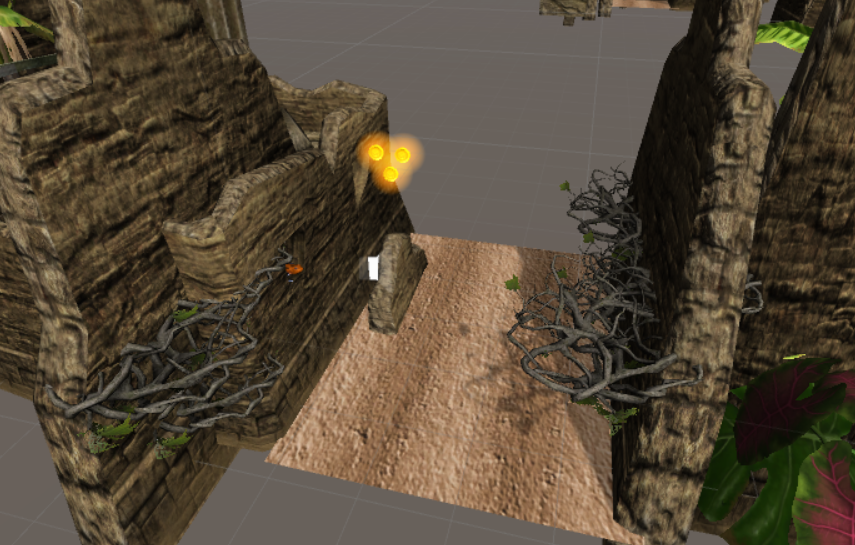
\includegraphics[width=0.85\textwidth]{LeftHandUp}
    \caption{Left hand up segment.}
    \label{fig:leftup}
\end{figure}
\begin{figure}[h]
    \centering
    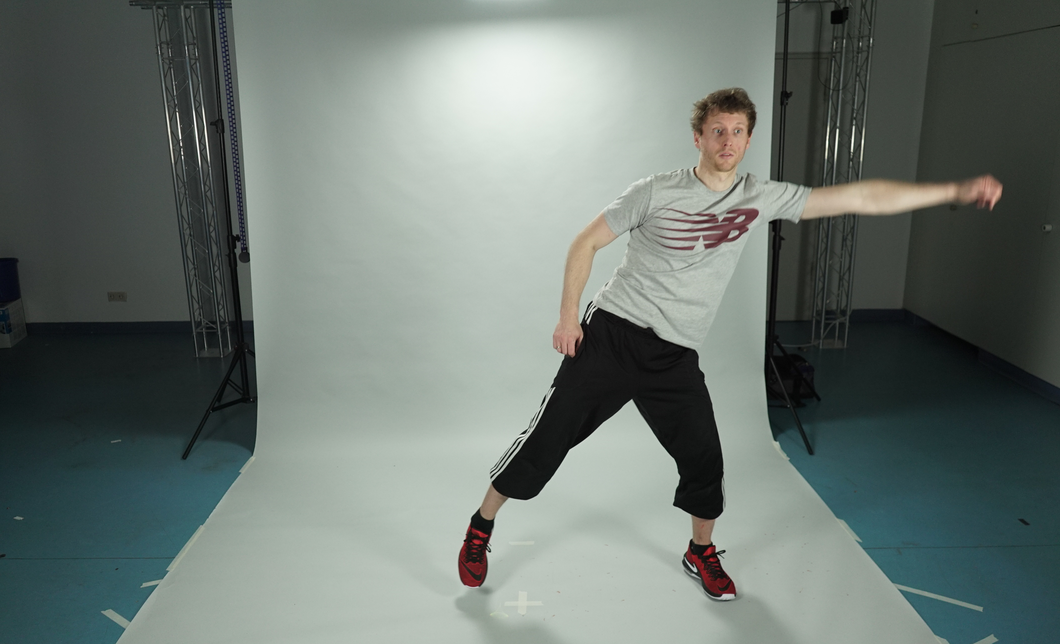
\includegraphics[width=0.85\textwidth]{ExpertLeftHandUp}
    \caption{Expert left hand up movement.}
    \label{fig:leftHandUp}
\end{figure}\\
In segments presented in Figure \ref{fig:wolfRight} and Figure \ref{fig:goblin} similar hand movements were required to be performed. The only difference was that in these segments the user is given a choice whether to go left or right. \\For instance, in Figure \ref{fig:goblin} player could collect four coins by moving to the right side. On the other hand, the player could also chose to go left and collect a blue coin that was worth five points. However, there was a possibility to lose points if collided with the obstacle.\\
\begin{figure}[h]
    \centering
    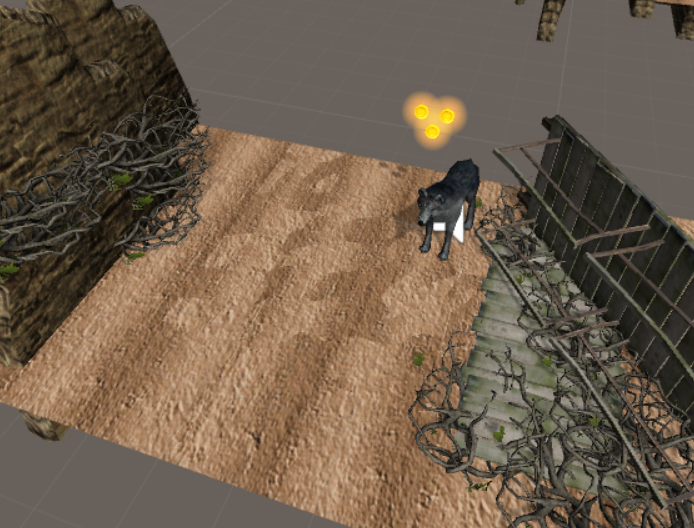
\includegraphics[width=0.85\textwidth]{HandUpRightWolf}
    \caption{Right hand up segment.}
    \label{fig:wolfRight}
\end{figure}
\begin{figure}[h]
    \centering
    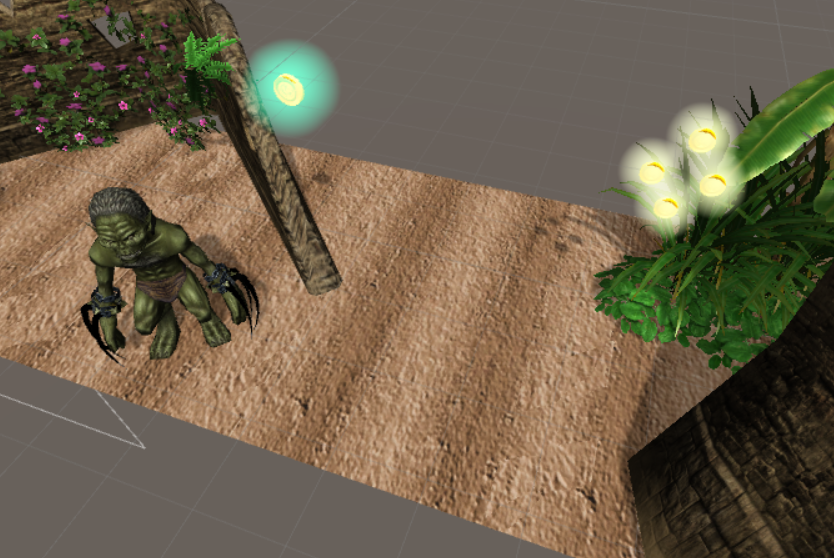
\includegraphics[width=0.85\textwidth]{GoblinHandLeftOrRight}
    \caption{Right or Left hand up with goblin segment.}
    \label{fig:goblin}
\end{figure}\\\\
Figures \ref{fig:2wolfs} and Figure \ref{fig:2sides} show segments in which the player was also given an option to chose which movement to perform. Both the movements included rising hand in the upper position. The decision was left to the player. In case the player opted for the left side, the possible reward were two blue coins that were worth ten points in total. In case the player opted for the right side, the possible reward were three red coins that were worth nine points in total. However, there was a possibility to lose points by colliding with the obstacle.\\
\begin{figure}[h]
    \centering
    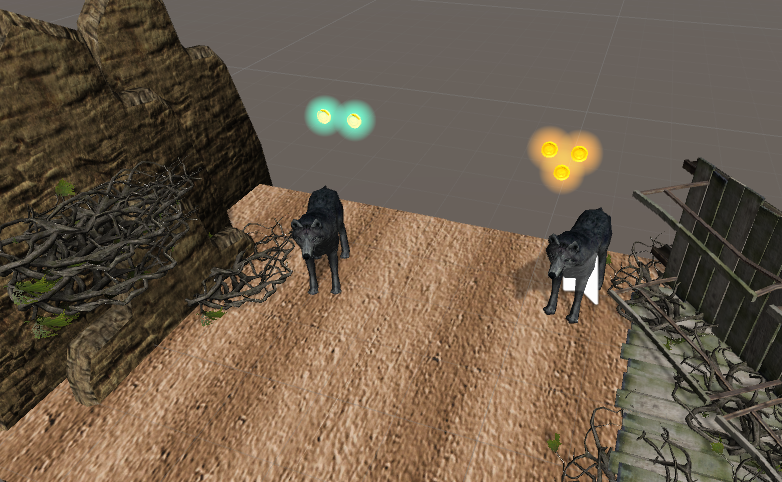
\includegraphics[width=0.85\textwidth]{2WolfsRight}
    \caption{Right or Left hand up with two wolfs segment.}
    \label{fig:2wolfs}
\end{figure}\\
\begin{figure}[h]
    \centering
    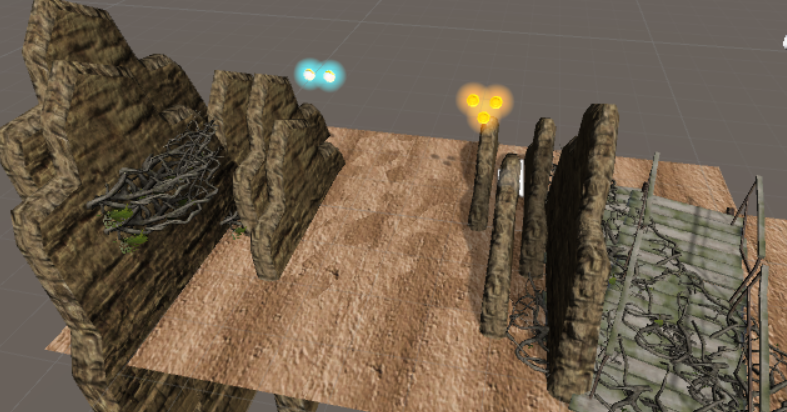
\includegraphics[width=0.85\textwidth]{TwoSides}
    \caption{Right or Left hand up with walls segment.}
    \label{fig:2sides}
\end{figure}\\\\
In Figure \ref{fig:jumpleft} the player was required to move to the left and touch the floor with the left hand in order to collect the coins. Moreover, the player was required to stay in that position for a short amount of time in order to collect all the coins and than move to the right in order to avoid the obstacle.
\begin{figure}[h]
    \centering
    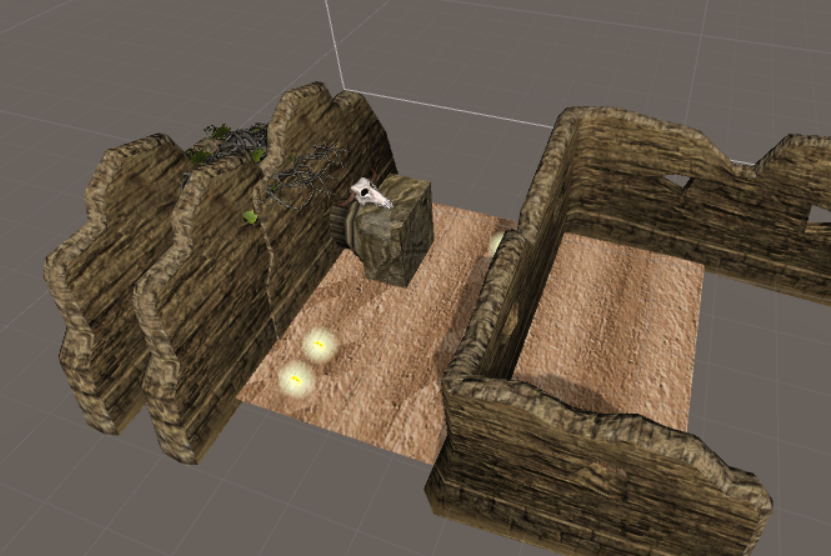
\includegraphics[width=0.85\textwidth]{JumpRight}
    \caption{Move left segment.}
    \label{fig:jumpleft}
\end{figure}
\begin{figure}[h]
    \centering
    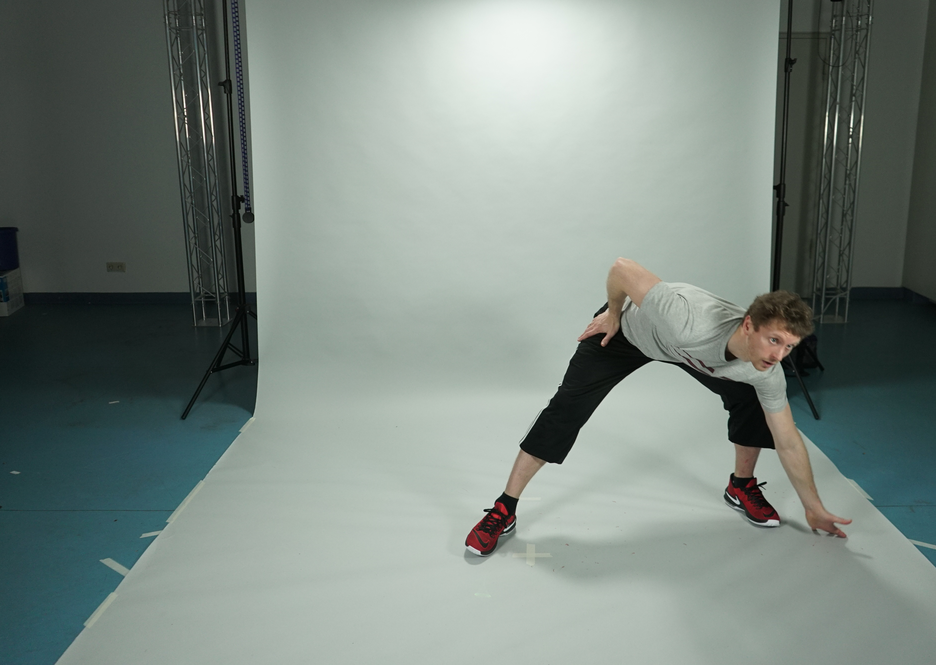
\includegraphics[width=0.85\textwidth]{ExpertHandDownLeft}
    \caption{Expert left hand down movement.}
    \label{fig:expertLeftDown}
\end{figure}\\
In Figure \ref{fig:jumpright} the player was required move to the right and touch the floor with the right hand in order to collect the coins. As in previous segments, in case an obstacle was hit, the overall score was reduced by one.\\
\begin{figure}[h]
    \centering
    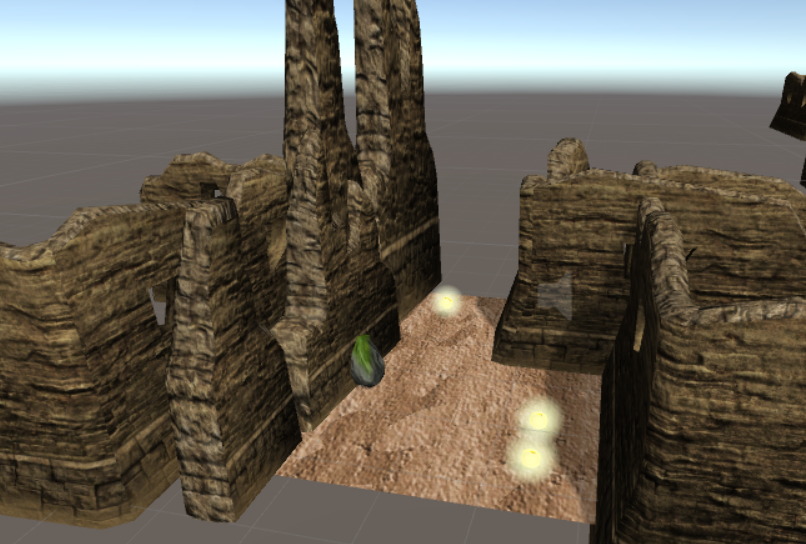
\includegraphics[width=0.85\textwidth]{JumpLeft}
    \caption{Move right segment.}
    \label{fig:jumpright}
\end{figure}
\begin{figure}[h]
    \centering
    \includegraphics[width=0.85\textwidth]{ExpertHandDownRight}
    \caption{Expert right hand down movement.}
    \label{fig:expertLeftDown}
\end{figure}\\\\
In the segment presented in Figure \ref{fig:rightleft} the player was required to move right then left. Compared to the similar movements depicted in previous figures, the movements in this segment needed to be performed much faster in order to collect the coins and avoid obstacles.\\
\begin{figure}[h]
    \centering
    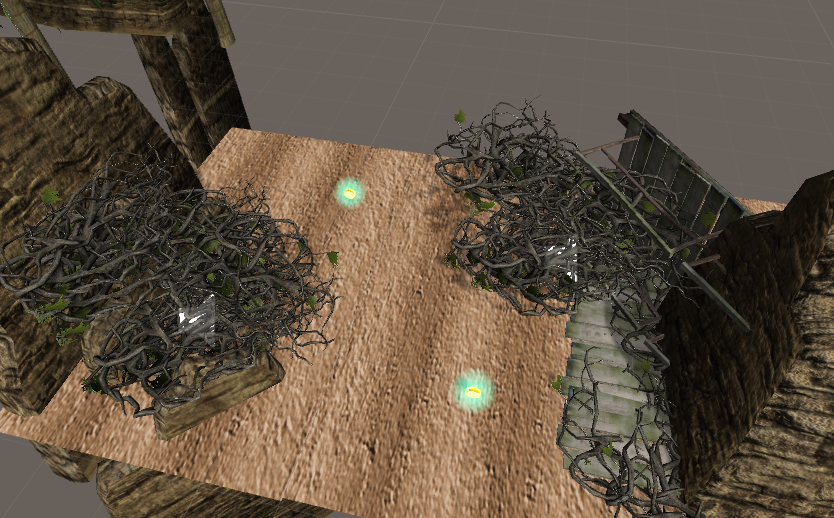
\includegraphics[width=0.85\textwidth]{RightLeft}
    \caption{Move right and left segment.}
    \label{fig:rightleft}
\end{figure}
\begin{figure}[h]
    \centering
    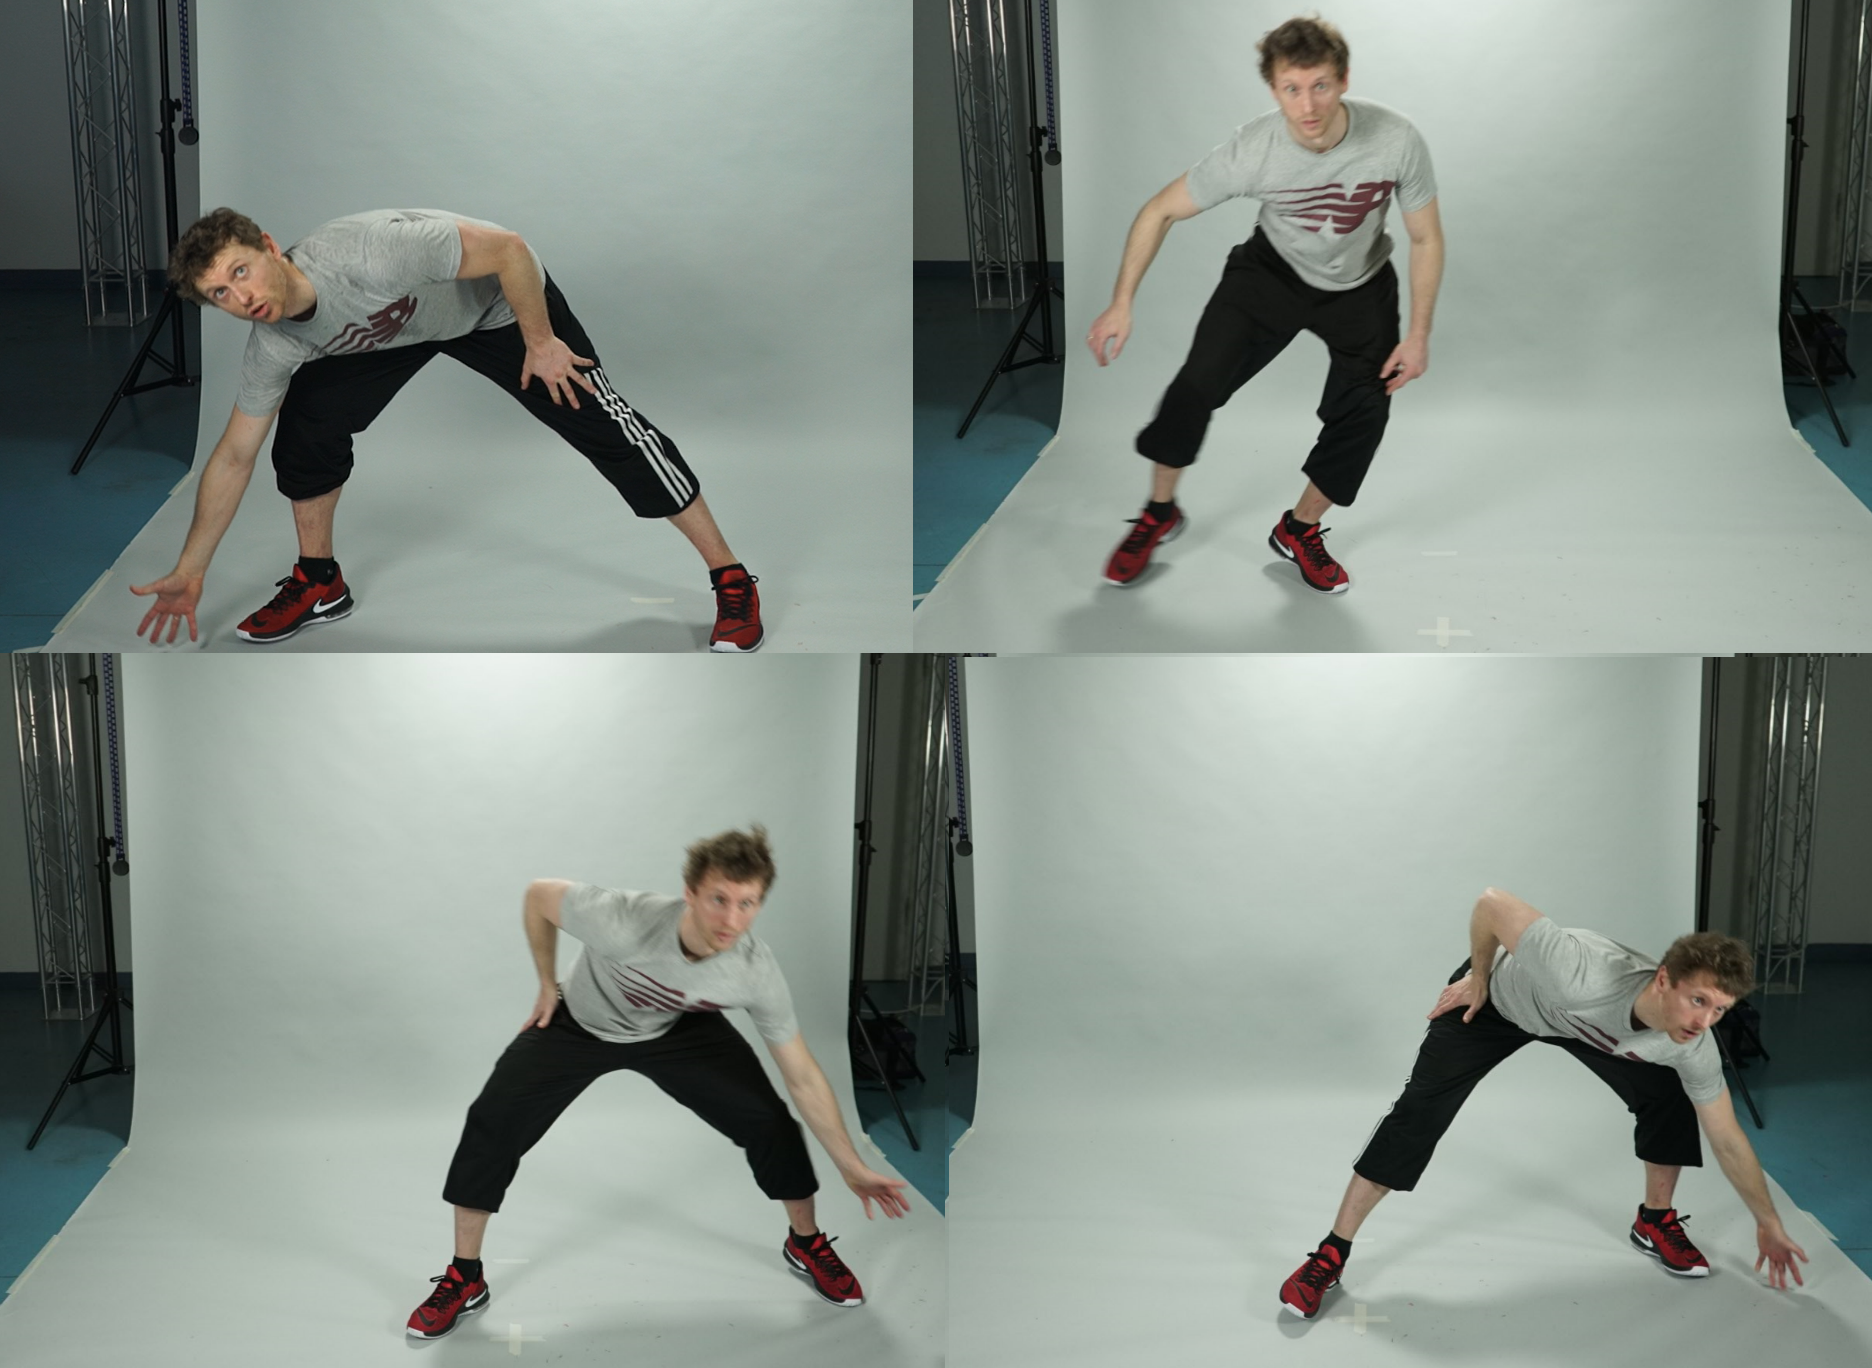
\includegraphics[width=0.85\textwidth]{ExpertLeftRight}
    \caption{Expert right and left movement.}
    \label{fig:expertLeftRight}
\end{figure}\\
Figure \ref{fig:squatleft} and Figure \ref{fig:squatright} show game segments in which the player was required to move right or left as in segments showed in Figure \ref{fig:jumpleft} and Figure \ref{fig:jumpright}. The main difference is that after moving right or left, additional squat is required in order to avoid the obstacle and collect the coins. The obstacle was placed above the the coins, and in case the player hit one of the obstacle, the overall score was reduced by one.\\
\begin{figure}[h]
    \centering
    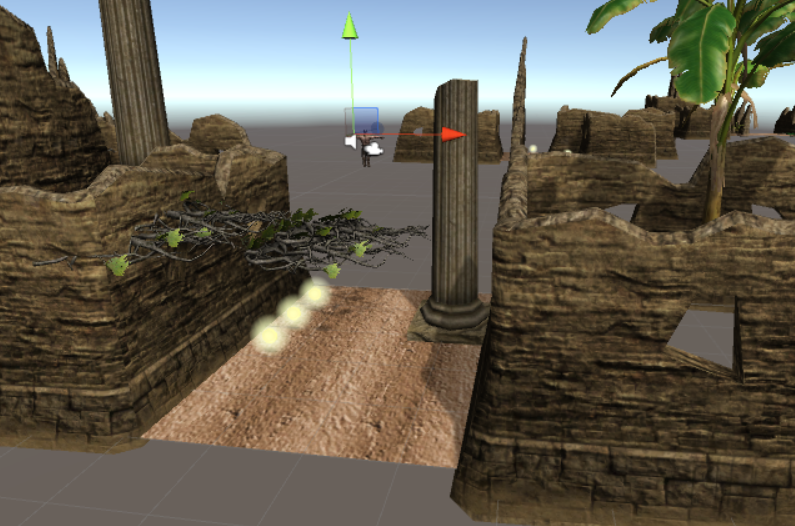
\includegraphics[width=0.9\textwidth]{SquatLeft}
    \caption{Move left and squat segment.}
    \label{fig:squatleft}
\end{figure}\\
\begin{figure}[h]
    \centering
    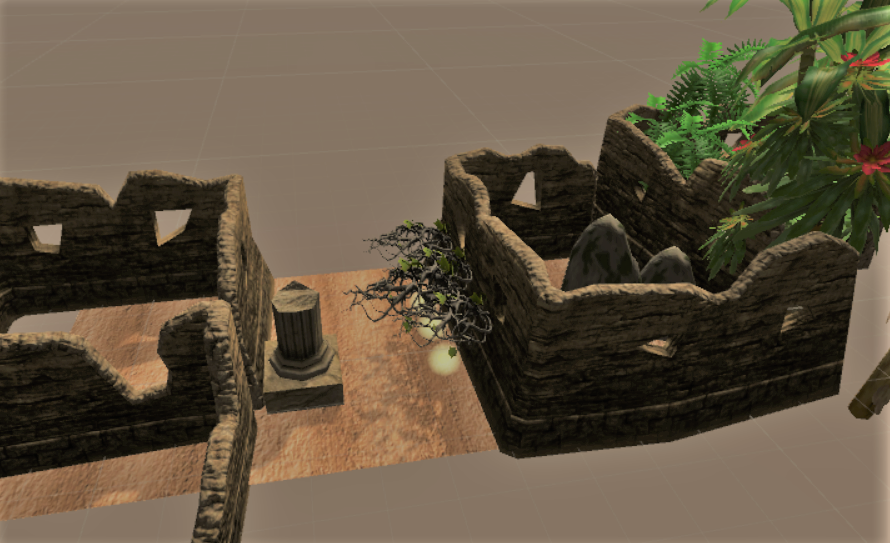
\includegraphics[width=0.9\textwidth]{SquatRight}
    \caption{Move right and squat segment.}
    \label{fig:squatright}
\end{figure}\\
In Figures \ref{fig:jumpup} and Figure \ref{fig:jumpssmallrock}, the player was required to perform a jump in order to avoid the obstacle and collect the coins. The obstacle depicted in Figure \ref{fig:jumpup} was the lowest in the middle and in case it was hit, the player's total score was reduced by one point. The player was presented with a choice of collecting additional blue coins with the jump. The blue coins were positioned in a way that required higher jump and placing both hand in the upper position in order to be collected.\\
\begin{figure}[h]
    \centering
    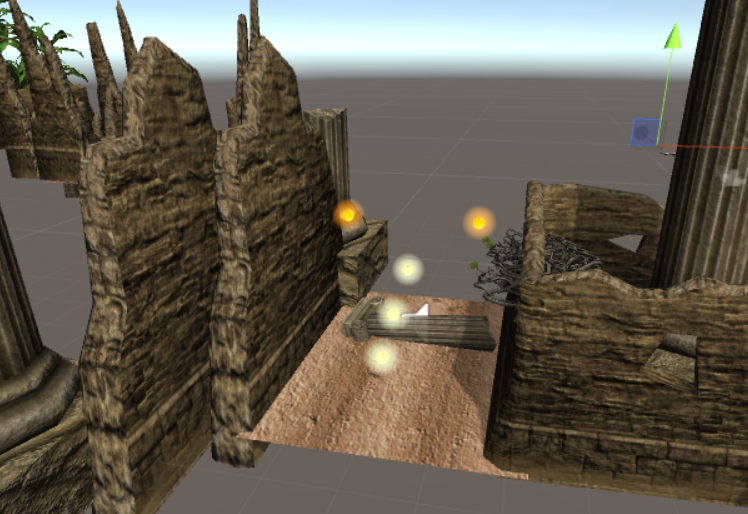
\includegraphics[width=0.85\textwidth]{JumpUp}
    \caption{Jump up segment.}
    \label{fig:jumpup}
\end{figure}\\
Compared to the movement required in the previous segment, the one needed to be executed in Figure \ref{fig:jumpssmallrock} did not require additional hand movement.\\
\begin{figure}[h]
    \centering
    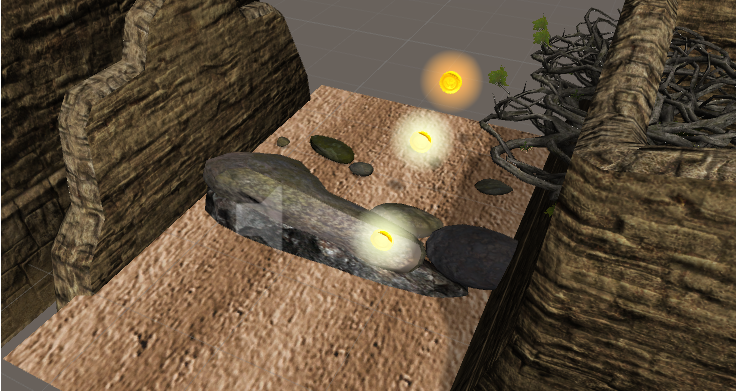
\includegraphics[width=0.85\textwidth]{JumpSmallRock}
    \caption{Jump up segment.}
    \label{fig:jumpssmallrock}
\end{figure}\\
Figure \ref{fig:star} depicts a game segment where the player was required to perform a \textit{star} jump in order to collect all the coins.\\
\begin{figure}[h]
    \centering
    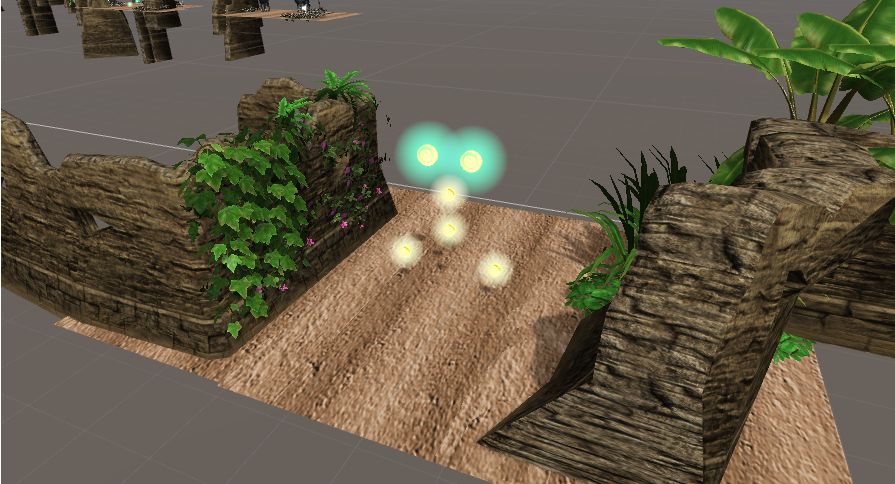
\includegraphics[width=0.85\textwidth]{JumpinJack}
    \caption{Star jump segment.}
    \label{fig:star}
\end{figure}
\begin{figure}[h]
    \centering
    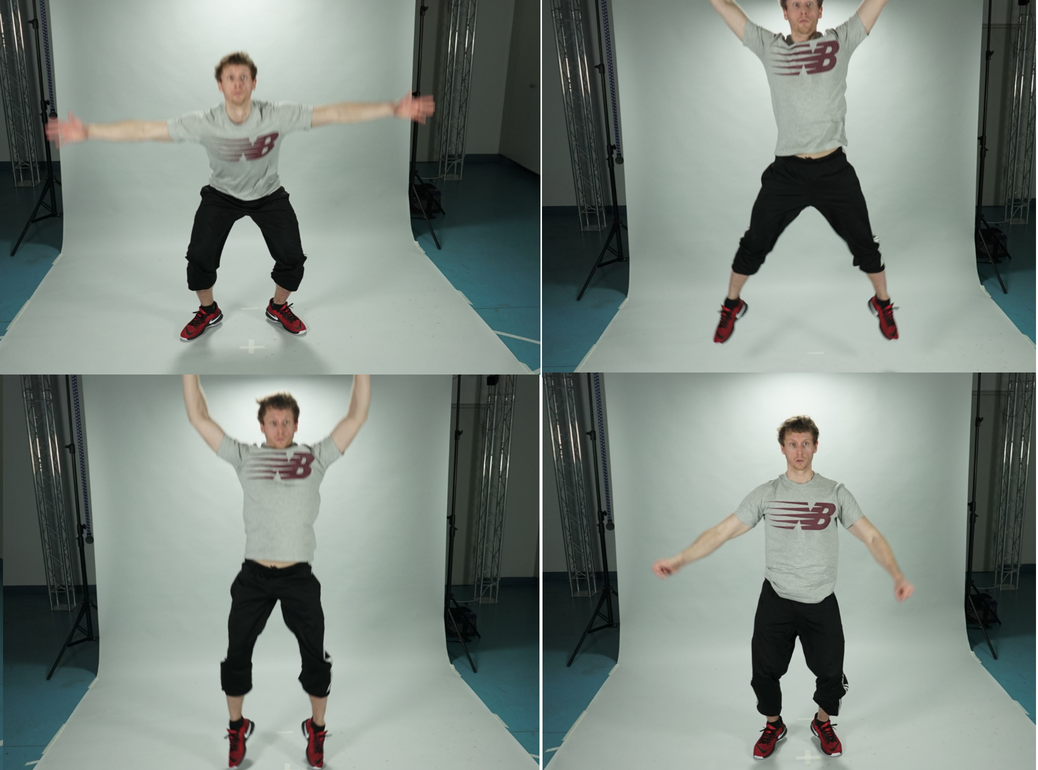
\includegraphics[width=0.85\textwidth]{ExpertJump}
    \caption{Star jump movement.}
    \label{fig:expertstarjump}
\end{figure}\\\\\\\\
Figures \ref{fig:squat} and Figure \ref{fig:squatlong} depict game segments in which the player was required to perform a squat in order to collect coins and avoid the obstacle. In case the user hit the obstacle placed above the coins, the overall score was reduced by one point.\\
\begin{figure}[h]
    \centering
    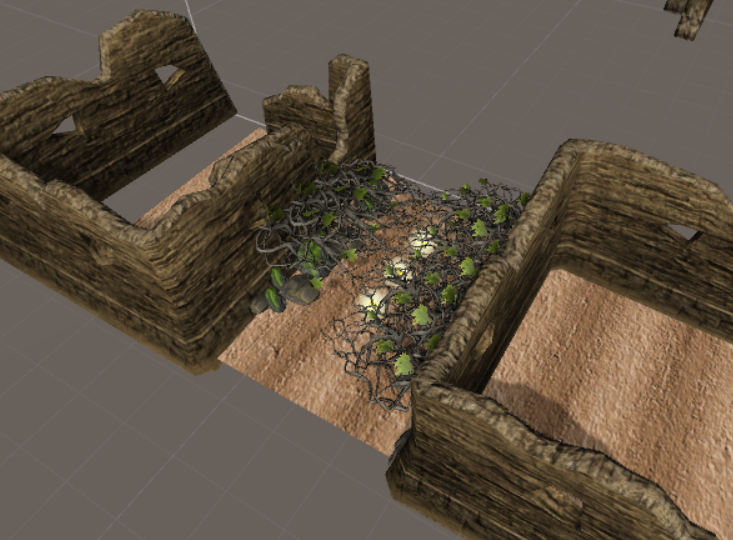
\includegraphics[width=0.85\textwidth]{Squat}
    \caption{Squat segment.}
    \label{fig:squat}
\end{figure}
\begin{figure}[h]
    \centering
    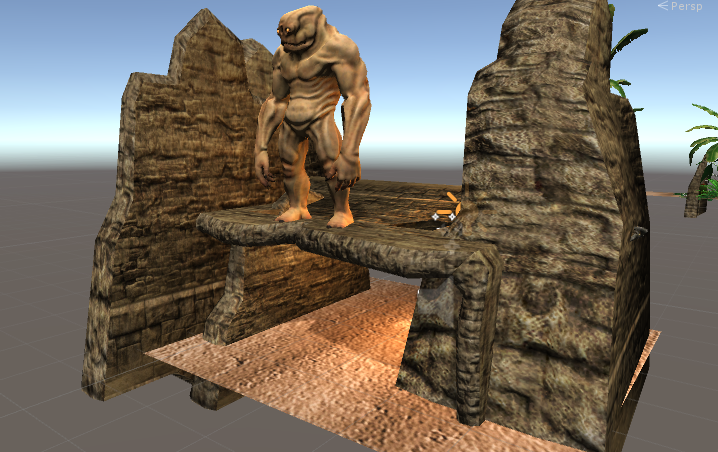
\includegraphics[width=0.85\textwidth]{SquatLong}
    \caption{Squat long segment.}
    \label{fig:squatlong}
\end{figure}\\
\begin{figure}[h]
    \centering
    \includegraphics[width=0.85\textwidth]{ExpertSquat}
    \caption{Squat movement.}
    \label{fig:squatlong}
\end{figure}\\
Figure \ref{fig:bridge} is one of the filler segments used for the player to prepare for the next movement. However, in case the player did not use the bridge and came in contact with the walls or lava obstacles, the overall score was reduced by one point.
\begin{figure}[h]
    \centering
    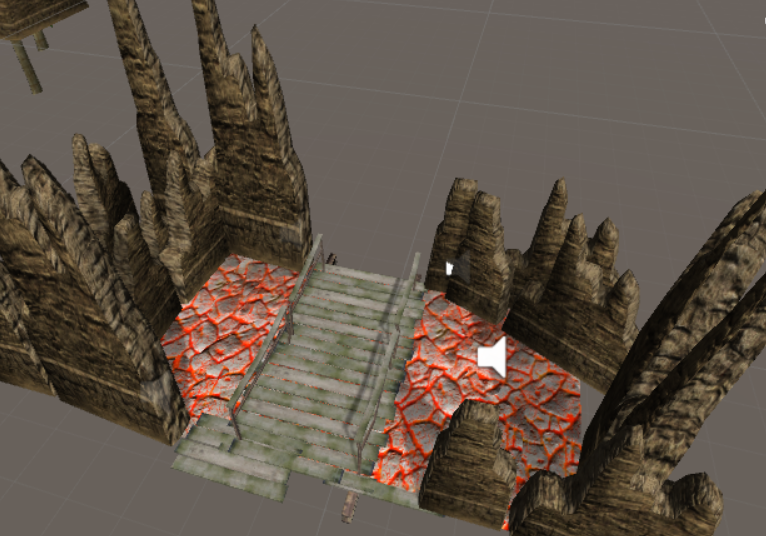
\includegraphics[width=0.85\textwidth]{Bridge}
    \caption{Bridge segment.}
    \label{fig:bridge}
\end{figure}\\
Figure \ref{fig:filler} depicts the rest of the filler segments that are placed at the beginning of the game and in between segments with obstacles in order to give players enough time to prepare for the subsequent movement.
\begin{figure}[h]
    \centering
    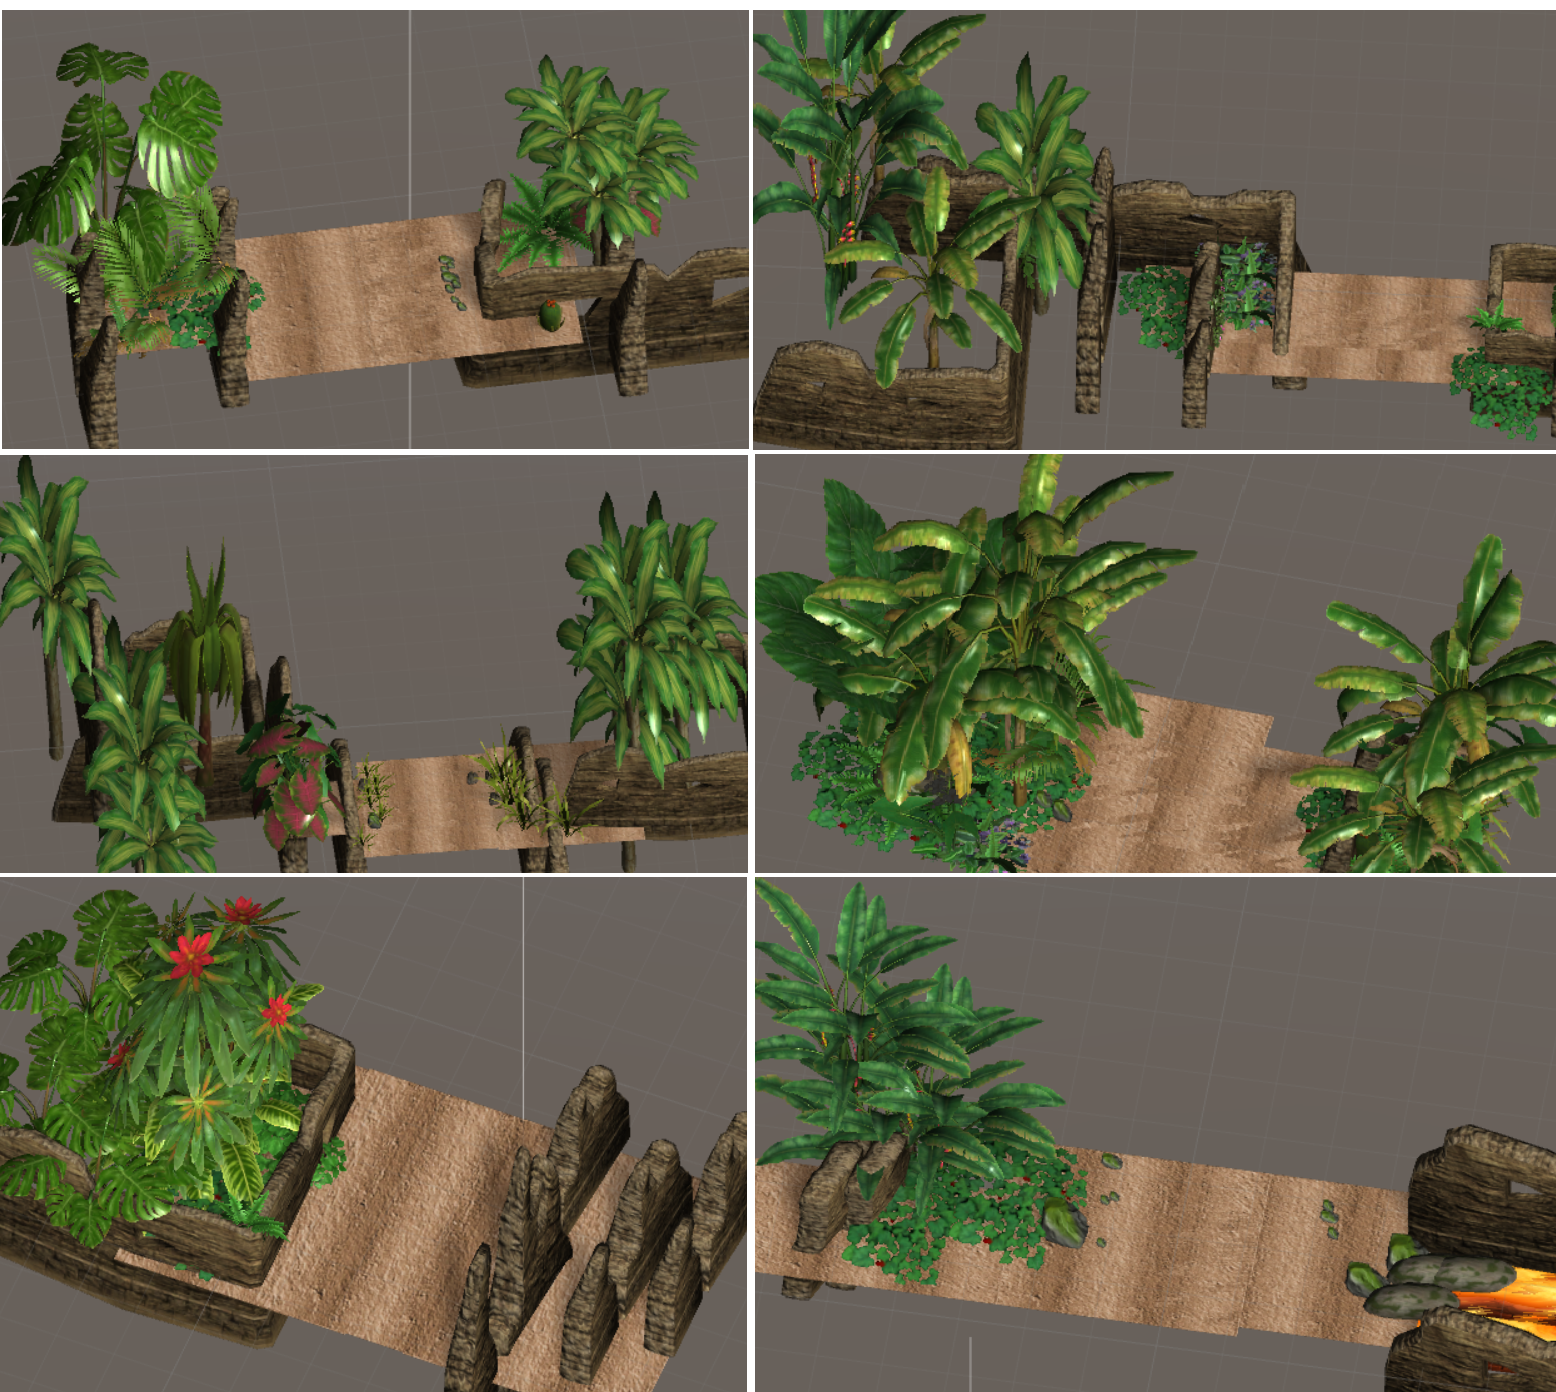
\includegraphics[width=\textwidth]{Filler1}
    \caption{Filler segments.}
    \label{fig:filler}
\end{figure}\\
To conclude, by placing the obstacle and coins in a specific position, our intention was to indirectly promote exercise through the gameplay of repeatedly performing warm up related movements chosen during previous development phases and discussions with fitness experts. We ought to design game segments that are engaging for the player so we immerse the exergame players sufficiently so that their focus is shifted from the discomfort and exertion of the exercise towards the enjoyment of the experience.\pagebreak
\section{Game End Overview}
We implemented two approaches for ending the game. First one allowed the player to choose from a set of recommended warm up duration at the beginning of the gameplay. That is, the exergame ended after the selected time interval. The second was to end the exergame when the player felt warmed up enough for the subsequent physical activity. For the purpose of the user study, we utilized the second approach. This gave us information about the most common duration of the warm up sessions and later allowed us to compare it with the reported ones from self reported surveys. \\When the game ended, the \textit{Individual scoreboard} was presented to the player. The scoreboard is depicted in Figure \ref{fig:individualend}.\\
\begin{figure}[h]
    \centering
    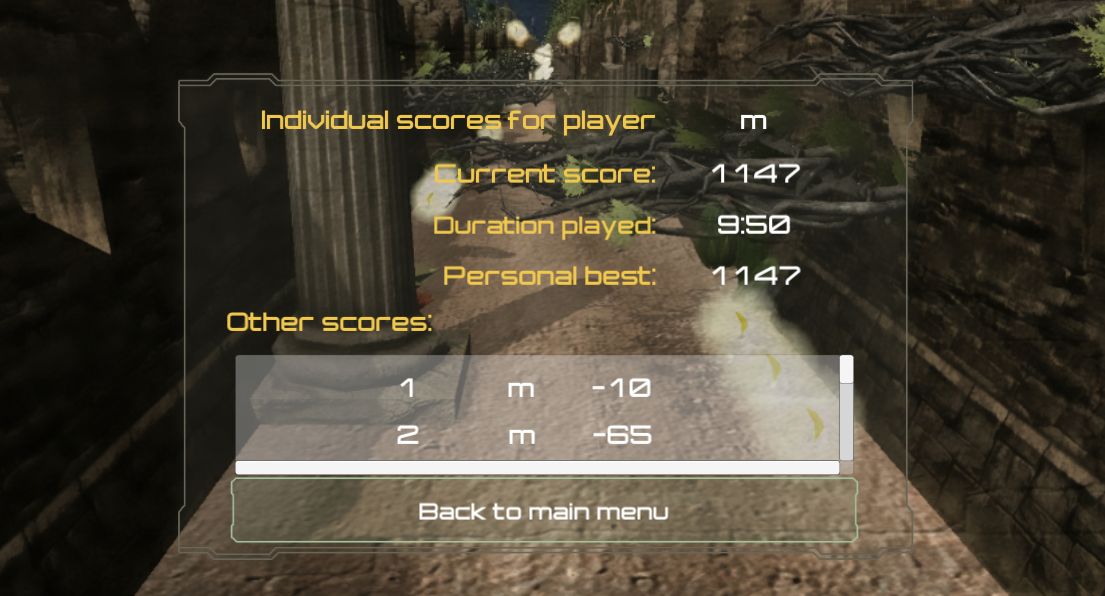
\includegraphics[width=\textwidth]{IndividualEndScene}
    \caption{Individual end scene.}
    \label{fig:individualend}
\end{figure}\\
Based on the player's username we displayed all the previous scores. The scores were displayed in descending order by the points achieved during each game run. The player was also presented with the duration each game lasted and the personal best score. By selecting the \textit{Back to main menu} button, the player could go back to the Home screen. 
\label{endgamelabel}
